\documentclass{article}
\usepackage{titling}
\usepackage{graphicx}
\usepackage[margin=1in]{geometry}
\usepackage{float}
\usepackage{caption}
\usepackage{subcaption}

\title{CM30225 Parallel Computing
Assessed Coursework Assignment 1}
\preauthor{}
\author{}
\postauthor{}

\begin{document}

\maketitle
\section{Algorithm Design}
My initial design for the algorithm was possibly too naiive; the plan was for all threads to work on the same given matrix, and simply lock the cells that they needed for the calculation whilst in use. 
    \begin{figure}[H]
        \centering
        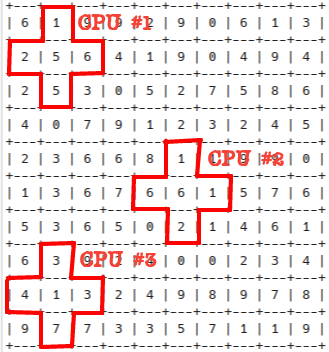
\includegraphics[scale=0.5]{1.png}
        \caption{Naiive Appoach}
        \label{fig1}
    \end{figure}
As can be seen in Figure \ref{fig1}, a thread would lock the current cell, and the cells required to decide the new average, until the calculation was complete. The thread then releases the lock and finds a new cell. Initially, this appears like it would be an acceptable solution, however on reflection, I realized that more time would be spent on overhead - locking cells, checking the status of cells, finding new unlocked cells - than would actually be spent on the main calculation. Thus I decided to find a new algorithm with higher work efficiency, and what follows is the solution I came to.\\
\begin{figure}
    \centering
    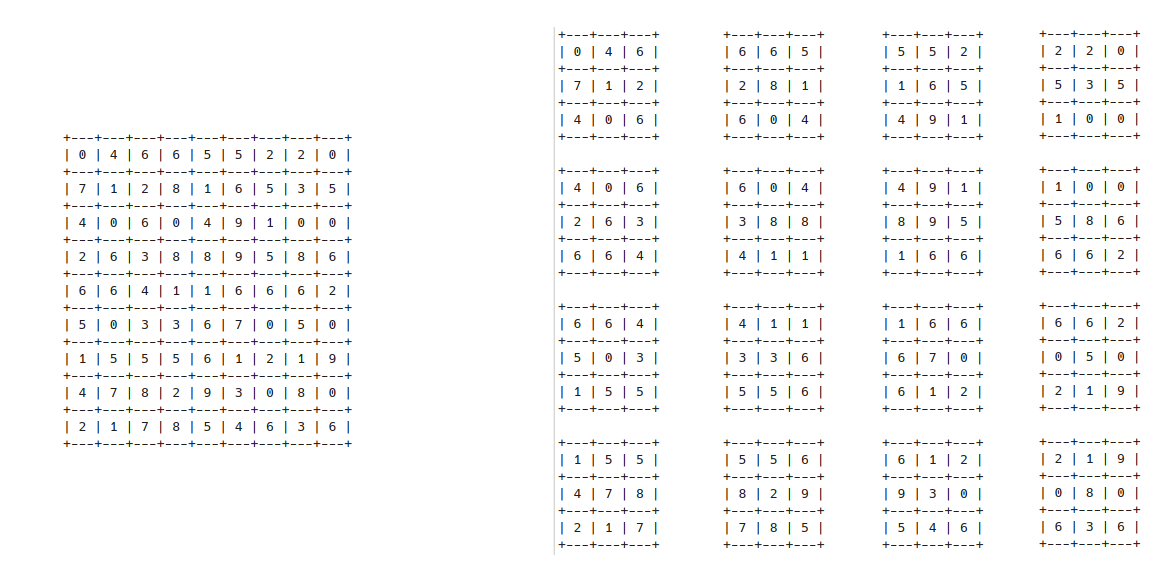
\includegraphics[scale=1.6]{2.png}
    \caption{Scalable Approach}
    \label{fig2}
\end{figure}
\begin{figure}
    \centering
    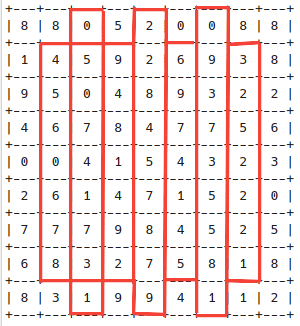
\includegraphics[scale=0.5]{3.png}
    \caption{Boundary computation: First columns, then rows}
    \label{fig3}
\end{figure}
In Figure \ref{fig2}, the matrix is split into \textit{p} sub-matrices, where \textit{p} is the number of processors the program is to run on, and each sub-matrices boundary overlaps its neighbours (In Figure \ref{fig2}, it is assumed there are 16 processors to run on). The process runs as expected, with each thread computing the inner values of its matrix to the desired precision, and leaving the boundaries untouched.
Then sub-matrices will be merged, and their boundaries computed. If the initial matrix is of an odd size (i.e. 9x9), their boundaries will be computed as a $3*n$ array, where $n$ is the size of the $n*n$ square array provided. The first pass will be columns, and then second pass is rows (See Figure \ref{fig3}). For even arrays, one set of sub-matrices will have an extra column/row, so computation will be marginally slower for even arrays.\\
As seen in Figure \ref{fig3}, The arrays passed to each processor will overlap, however since the shared values have already been computed to the desired precision and won't be changed, this shouldn't cause any issues. \\
This is my initial consideration of the algorithm design, pre-development. There is obviously room for improvement; for example, if the number of processors \textit{p} does not evenly fit into the $(n+1)^2$ sub-matrices generated (as in Figure \ref{fig2}), what should be done? Clearly, the division of the matrix into an efficient number of sub-matrices can be improved, however I maintain that this principle of overlapping sub-matrices and then subsequently computing boundaries along columns/rows appears to be a good approach.
\subsubsection{Final Algorithm}
After much painstaking deliberation, what I believe to be the optimal algorithm has been found. It is a halfway compromise between the initial random-find-and-lock algorithm and the overly complicated divide-and-conquer algorithm.\\
\begin{figure}
    \centering
    \begin{subfigure}{.5\textwidth}
      \centering
      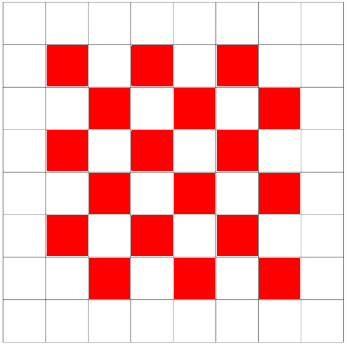
\includegraphics[width=.4\linewidth]{4.png}
      \caption{First Pass}
      \label{fig:sub1}
    \end{subfigure}%
    \begin{subfigure}{.5\textwidth}
      \centering
      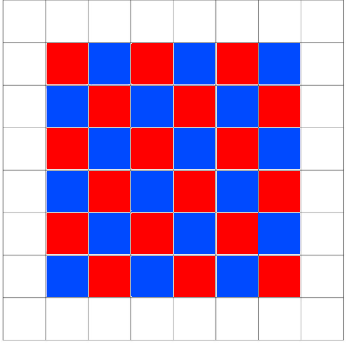
\includegraphics[width=.4\linewidth]{5.png}
      \caption{Second Pass}
      \label{fig:sub2}
    \end{subfigure}
    \caption{Matrix Passes of the Algorithm}
    \label{fig4}
    \end{figure}
As can be seen in figure \ref{fig4}, If the diagonals of the matrix are taken, and the red cells have their values calculated, there is no interference between threads. In the second pass, the opposite diagonals are calculated, and the computation is complete. The intuitive way to perform this calculation is as follows:
\begin{enumerate}
    \item The diagonal cells in Figure \ref{fig:sub1} are identified; this is Pass \#1
    \item The diagonal cells in Figure \ref{fig:sub2} are identified. this is Pass \#2
    \item The number of items in Pass \#1 is divided by the number of threads for the process to run on. This gives us the number of cells each thread must process, $n$.
    \item The same is done for Pass \#2, $m$.
    \item Each thread is randomly assigned $n$ exclusive items from Pass \#1, and $m$ items for Pass \#2.
    \item The cells in Pass \#2 are locked with a singular mutex.
    \item The threads perform their calculations to the desired precision.
    \item Threads submit a message to a control thread when they have completed their computation.
    \item Threads poll the mutex lock waiting. 
    \item Once all threads have completed their computations, the control thread unlocks the cells for Pass\#2.
    \item Once the cells are unlocked, the threads are free to complete the computations on their assigned Pass \#2 cells.
\end{enumerate}
This algorithm at first glance appears to elegantly avoid all race conditions and maximise the work throughput of threads.
\end{document}
